% Standalone source. Compile twice with pdflatex or xelatex.
% All figure coordinates and bibliography entries are embedded below.
\documentclass[11pt,letterpaper]{article}
\ifdefined\pdfinfoomitdate\pdfinfoomitdate=1\fi
\ifdefined\pdftrailerid\pdftrailerid{}\fi
\ifdefined\pdfsuppressptexinfo\pdfsuppressptexinfo=15\fi
\usepackage[T1]{fontenc}
\usepackage[utf8]{inputenc}
\usepackage{newtxtext,newtxmath}
\usepackage[margin=0.82in,top=0.75in,bottom=0.75in]{geometry}
\usepackage{microtype}
\usepackage{booktabs}
\usepackage{amsmath}
\usepackage{graphicx}
\usepackage{pgfplots}
\usepackage{caption}
\usepackage{float}
\usepackage{titlesec}
\usepackage[hidelinks]{hyperref}
\pgfplotsset{compat=1.18}
\hypersetup{pdftitle={Effects of Cognitive Impairment on Alpha-Band Power Modulation},pdfauthor={Kimia Fakheri}}
\definecolor{healthy}{HTML}{24627B}
\definecolor{impaired}{HTML}{A4512D}
\captionsetup{font=small,labelfont=bf,skip=7pt}
\titleformat{\section}{\large\bfseries}{\thesection}{0.6em}{}
\titlespacing*{\section}{0pt}{13pt}{6pt}
\setlength{\parindent}{1em}
\setlength{\parskip}{2pt}
\setlength{\textfloatsep}{13pt}
\setlength{\floatsep}{12pt}
\renewcommand{\topfraction}{0.9}
\renewcommand{\bottomfraction}{0.85}
\renewcommand{\textfraction}{0.08}
\renewcommand{\floatpagefraction}{0.72}
\setcounter{topnumber}{3}
\setcounter{bottomnumber}{2}
\emergencystretch=1.5em
\widowpenalty=10000
\clubpenalty=10000
\pagestyle{plain}

\begin{document}
% TITLE-BEGIN
\begin{center}
{\fontsize{16}{19}\selectfont\bfseries Effects of Cognitive Impairment on Alpha-Band Power Modulation\par}
\vspace{6pt}
{\normalsize Kimia Fakheri}
\end{center}
\vspace{3pt}
% TITLE-END
\fontsize{10.5}{12.4}\selectfont


\section*{Abstract}
\noindent The study examined changes in electroencephalographic (EEG) power across successive intervals of an auditory trial in healthy older adults and older adults diagnosed with mild cognitive impairment or mild Alzheimer's disease, assessing whether the two groups differed in the temporal pattern of power modulation. The analysis included EEG recordings from 20 participants, with 10 participants in each group, and used data from 25 auditory trials and 19 electrodes for each participant. To quantify how alpha (8 to 13 Hz) and gamma (39 to 41 Hz) power varied within auditory trials comprising 3 s of sound followed by 3 s without stimulation, a contrast was calculated for each participant and electrode by subtracting the mean log spectral density in the second onset-aligned analysis window from that in the first. Alpha contrasts differed significantly between groups at six electrodes after Benjamini-Hochberg correction (adjusted \(p=0.0283\) to \(0.0472\)). The reported group averages showed that alpha power was higher in the first analysis window than in the second for the healthy group, while the clinical group showed the reverse pattern, although comparisons of alpha power within either window and of gamma power contrasts did not detect significant differences between the groups. These findings identify a difference in alpha power modulation between the healthy and clinical groups and suggest that the clinical group's relatively greater alpha power in the later trial interval reflects a change in the temporal organization of neural activity during the auditory task.

\section{Introduction}
Prior literature has associated alpha modulation with the selection of task-relevant sounds and the suppression of distractors, thereby linking changes in this band to attentional processes that prioritize relevant auditory information and regulate interference from competing input. After rhythmic auditory stimulation, Ronconi et al. found that greater alpha activity before a visual attentional-blink task was associated with more successful target detection \cite{ronconi}, while W\"ostmann et al. identified distinct alpha responses during the selection of relevant sounds and the suppression of distractors \cite{wostmann}, illustrating how alpha activity relates to different aspects of attention, from detecting a target to controlling which sounds receive attention. While these alpha findings concern the control of attention, Van Deursen et al. examined auditory activity in relation to clinical status, reporting higher 40 Hz auditory steady-state response power in mild Alzheimer's disease than in mild cognitive impairment or healthy aging under periodic auditory stimulation \cite{vandeursen}.

These findings provide a basis for the hypothesis that the attentional processes involved in selecting relevant sounds and suppressing distractors differ between healthy older adults and adults with mild cognitive impairment or mild Alzheimer's disease, motivating an examination of alpha power modulation across successive auditory trial intervals. EEG recordings during an auditory trial provide information about both power within an interval and its change across successive intervals, with a within-participant contrast expressing that change as the difference between each participant's two window measurements. Comparing these contrasts between groups tests differences in temporal modulation directly, while retaining the pairing of the two measurements and complementing separate-window comparisons that address the power present at each stage of the trial.

The clinical findings on 40 Hz responses also motivate including gamma alongside alpha in the comparison of temporal power modulation, with the present analysis measuring gamma band power rather than a stimulus-locked auditory steady-state response. The analysis compared alpha and gamma power contrasts between healthy older adults and the clinical group to test whether power changed differently across the two consecutive onset-aligned windows, while separate comparisons of alpha power within each window assessed between-group differences in the two measurements used to calculate the contrast. As each trial comprised sound presentation followed by a period without stimulation, the contrasts were interpreted in relation to both activity associated with the sound and activity later in the trial, either of which could contribute to a difference between groups.

\section{Methods}
Under the clinical protocol, inclusion in either group required a minimum age of 60 years and a thorough cognitive assessment by a licensed neurologist, including examinations such as the Mini-Mental State Examination (MMSE). Following assessment, 10 age-eligible adults diagnosed with mild cognitive impairment (MCI) or mild Alzheimer’s disease (AD) were classified as the Clinical group, while another 10 without measurable memory impairment were classified as the Healthy group. Exclusion criteria included schizophrenia, stroke, other neurological or neurodegenerative diseases, traumatic brain injury, and olfactory-pathway injury, along with advanced AD. Neurologist-diagnosed dementia was also grounds for exclusion, except for the cases of mild AD included in the Mild group. Individuals were also ineligible if visual or hearing impairments prevented adequate reception of stimuli, and the same applied to anyone who had received any pharmacological intervention or undergone brain stimulation within the preceding six months.

The protocol included an auditory task in which a single-frequency sound was presented for 3 s through the Synaptic device and a Bluetooth speaker, followed by 3 s without stimulation. The analysis used continuous EEG recordings from 25 trials per participant, acquired from 19 electrodes positioned according to the international 10-20 system together with an event-trigger channel.

Before spectral estimation, the event-trigger channel was removed and each electrode's signal was standardized using z-scores calculated separately for each participant, with trial onsets then adjusted by the participant-specific offsets of 0 to 2.0 s previously established for phase-locking alignment. The adjusted onset served as the reference for dividing each trial into a first window of 3.03 s and a second window of 2.97 s, and these window labels identify the intervals used for analysis, while “stimulation” and “post-stimulation” identify the nominal periods specified in the experimental protocol.

Welch's method provided a power spectral density estimate for every trial, electrode, and window, after which each estimate was transformed using \(10\log_{10}(P)\) \cite{welch} and averaged across trials before averaging across frequency bins within the alpha and gamma bands. The resulting band-power measure is the mean log spectral density of the standardized EEG signals, so contrasts between windows expressed in decibels describe differences in this measure on its logarithmic scale rather than differences in absolute EEG power.

The contrast for each participant, electrode, and band was
\begin{equation}
C = B_1 - B_2,
\label{eq:contrast}
\end{equation}
where \(B_1\) and \(B_2\) denote mean log spectral density in the first and second aligned windows, respectively, following the trial and frequency averaging described above. A positive contrast therefore indicates higher power in the first window, while a negative contrast indicates higher power in the second window.

Participants' contrasts were compared between groups using independent-samples \(t\)-tests at each electrode, with additional comparisons examining alpha power separately in each window. Benjamini-Hochberg (BH) adjustment was applied to each set of 19 alpha tests, treating the contrast and the two separate-window outcomes as distinct correction families \cite{bh}. All between-group tests used participant-level values, with alpha comparisons evaluated against a BH-adjusted threshold of \(p<0.05\) and gamma comparisons against an unadjusted threshold of \(p<0.05\). Paired \(t\)-tests compared the two windows within each group at the frontal, central, and parietal midline electrodes, while Wilcoxon signed-rank tests examined the same within-group differences as a rank-based sensitivity analysis. An unadjusted threshold of \(p<0.05\) applied to these additional tests, alongside 95\% confidence intervals for the mean paired differences that characterized the uncertainty in each group's midline contrast estimates.

\section{Results}
The change in alpha power between each participant's two aligned windows differed significantly between groups at six of the 19 electrodes after BH correction, with findings at frontal, temporal, central, and parietal recording positions (adjusted \(p\) values, \(0.0283\) to \(0.0472\), Table~\ref{tab:tests}). Comparisons of power within each window were nonsignificant at every electrode, with BH-adjusted \(p\) values of \(0.986\) throughout the first window and \(0.913\) throughout the second, so the significant findings concerned the paired changes between windows.

The frontal midline was among the six electrodes with a significant BH-corrected group difference, with Figure~\ref{fig:contrasts} showing a mean contrast of \(+0.26\) dB in healthy participants (95\% CI, \(-0.034\) to \(0.558\)) and \(-0.22\) dB in the clinical group (95\% CI, \(-0.505\) to \(0.057\)). The mean alpha estimates indicated higher power in the first window among healthy participants and in the second window among clinical participants, corresponding to a between-group separation of approximately \(0.48\) dB in the mean contrasts. For the healthy group, mean power was \(-15.54\) dB in the first window and \(-15.80\) dB in the second, whereas the clinical group showed corresponding means of \(-15.62\) and \(-15.39\) dB. Central and parietal midline estimates followed the same descriptive pattern, although their between-group comparisons did not reach significance after BH correction (adjusted \(p=0.1015\) and \(0.0822\), respectively).

\begin{figure}[H]
\centering
% FIGURE-DATA-BEGIN
% band|group|location|electrode|mean_db|lower_95ci|upper_95ci
% Alpha|Healthy|Frontal midline|Fz|0.26|-0.034|0.558
% Alpha|Healthy|Central midline|Cz|0.40|-0.018|0.822
% Alpha|Healthy|Parietal midline|Pz|0.29|-0.171|0.752
% Alpha|Clinical group|Frontal midline|Fz|-0.22|-0.505|0.057
% Alpha|Clinical group|Central midline|Cz|-0.05|-0.396|0.286
% Alpha|Clinical group|Parietal midline|Pz|-0.25|-0.594|0.094
% Gamma|Healthy|Frontal midline|Fz|0.14|-0.225|0.508
% Gamma|Healthy|Central midline|Cz|0.24|-0.265|0.738
% Gamma|Healthy|Parietal midline|Pz|0.29|-0.369|0.951
% Gamma|Clinical group|Frontal midline|Fz|0.01|-0.485|0.502
% Gamma|Clinical group|Central midline|Cz|0.03|-0.527|0.588
% Gamma|Clinical group|Parietal midline|Pz|0.23|-0.251|0.703
% FIGURE-DATA-END
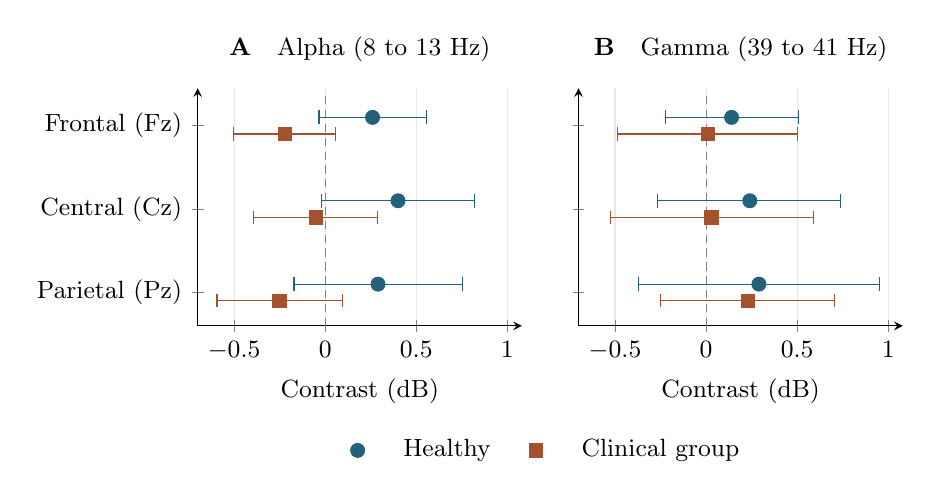
\begin{tikzpicture}
\begin{axis}[
name=alpha,width=0.47\textwidth,height=4.6cm,
title={\textbf{A}\quad Alpha (8 to 13 Hz)},
xmin=-0.7,xmax=1.08,ymin=0.6,ymax=3.45,
ytick={1,2,3},yticklabels={Parietal (Pz),Central (Cz),Frontal (Fz)},
xtick={-0.5,0,0.5,1},xlabel={Contrast (dB)},
tick label style={font=\small},label style={font=\small},title style={font=\small},
axis lines=left,xmajorgrids=true,grid style={gray!18},
legend style={font=\small,draw=none,at={(1.08,-0.43)},anchor=north,legend columns=2,column sep=12pt},
legend cell align=left]
\draw[densely dashed,gray] (axis cs:0,0.6)--(axis cs:0,3.4);
\addplot[only marks,mark=*,mark size=2.5pt,color=healthy,error bars/.cd,x dir=both,x explicit]
coordinates {(0.26,3.10) +=(0.298,0) -=(0.294,0) (0.40,2.10) +=(0.422,0) -=(0.418,0) (0.29,1.10) +=(0.462,0) -=(0.461,0)};
\addlegendentry{Healthy}
\addplot[only marks,mark=square*,mark size=2.4pt,color=impaired,error bars/.cd,x dir=both,x explicit]
coordinates {(-0.22,2.90) +=(0.277,0) -=(0.285,0) (-0.05,1.90) +=(0.336,0) -=(0.346,0) (-0.25,0.90) +=(0.344,0) -=(0.344,0)};
\addlegendentry{Clinical group}
\end{axis}
\begin{axis}[
at={(alpha.east)},anchor=west,xshift=0.72cm,
width=0.47\textwidth,height=4.6cm,
title={\textbf{B}\quad Gamma (39 to 41 Hz)},
xmin=-0.7,xmax=1.08,ymin=0.6,ymax=3.45,
ytick={1,2,3},yticklabels={},
xtick={-0.5,0,0.5,1},xlabel={Contrast (dB)},
tick label style={font=\small},label style={font=\small},title style={font=\small},
axis lines=left,xmajorgrids=true,grid style={gray!18}]
\draw[densely dashed,gray] (axis cs:0,0.6)--(axis cs:0,3.4);
\addplot[only marks,mark=*,mark size=2.5pt,color=healthy,error bars/.cd,x dir=both,x explicit]
coordinates {(0.14,3.10) +=(0.368,0) -=(0.365,0) (0.24,2.10) +=(0.498,0) -=(0.505,0) (0.29,1.10) +=(0.661,0) -=(0.659,0)};
\addplot[only marks,mark=square*,mark size=2.4pt,color=impaired,error bars/.cd,x dir=both,x explicit]
coordinates {(0.01,2.90) +=(0.492,0) -=(0.495,0) (0.03,1.90) +=(0.558,0) -=(0.557,0) (0.23,0.90) +=(0.473,0) -=(0.481,0)};
\end{axis}
\end{tikzpicture}
\caption{\textbf{Magnitude and uncertainty of midline power contrasts:} points show group means of the first-window minus second-window difference, with horizontal bars representing 95\% confidence intervals for these mean paired differences (\(n=10\) per group). Both panels use the same scale, and positive values indicate higher mean log spectral density in the first aligned analysis window. These intervals describe uncertainty within each group, while the direct between-group tests and their correction status are reported in Table~\ref{tab:tests}.}
\label{fig:contrasts}
\end{figure}

The mean gamma contrasts were positive at the frontal, central, and parietal midline in both groups, indicating higher mean gamma power in the first aligned window than in the second at these recording positions. Figure~\ref{fig:contrasts} places these estimates alongside the alpha contrasts on a shared scale, showing both the magnitude of the changes between windows and the uncertainty around each group's mean. Across all 19 electrodes, the between-group comparisons yielded unadjusted \(p\) values ranging from \(0.2095\) to \(0.9710\) (Table~\ref{tab:tests}), with none of the gamma contrast comparisons reaching statistical significance.

In the exploratory midline analyses, paired \(t\)-tests were nonsignificant in both bands, while the only nominal Wilcoxon findings occurred for alpha at the frontal and central midline in healthy participants (both unadjusted \(p=0.049\)).

\begin{table}[H]
\centering
\caption{\textbf{Between-group comparisons of aligned-window power contrasts:} each test compares participant-level differences between 10 healthy adults and 10 adults with mild cognitive impairment or mild Alzheimer's disease, with all 19 electrodes included. Bold values indicate alpha comparisons meeting the BH-adjusted \(p<0.05\) threshold, whereas the gamma column reports unadjusted values for the corresponding contrasts.}
\label{tab:tests}
\small
\setlength{\tabcolsep}{6pt}
\renewcommand{\arraystretch}{1.00}
\begin{tabular}[t]{lrrr}
\toprule
Electrode & Alpha \(p\) & Alpha BH \(p\) & Gamma \(p\) \\
\midrule
Fp1 & 0.2679 & 0.3181 & 0.3143 \\
F3 & 0.0032 & \textbf{0.0283} & 0.2095 \\
C3 & 0.0437 & 0.0822 & 0.7513 \\
P3 & 0.2882 & 0.3221 & 0.9262 \\
O1 & 0.0231 & 0.0549 & 0.7841 \\
F7 & 0.0094 & \textbf{0.0357} & 0.4236 \\
T3 & 0.0025 & \textbf{0.0283} & 0.7345 \\
T5 & 0.3355 & 0.3355 & 0.9163 \\
Fz & 0.0149 & \textbf{0.0472} & 0.6296 \\
Cz & 0.0721 & 0.1015 & 0.5426 \\
\bottomrule
\end{tabular}\hspace{18pt}
\begin{tabular}[t]{lrrr}
\toprule
Electrode & Alpha \(p\) & Alpha BH \(p\) & Gamma \(p\) \\
\midrule
Pz & 0.0476 & 0.0822 & 0.8593 \\
Fp2 & 0.1047 & 0.1326 & 0.4394 \\
F4 & 0.3132 & 0.3306 & 0.9051 \\
C4 & 0.0077 & \textbf{0.0357} & 0.7304 \\
P4 & 0.0045 & \textbf{0.0283} & 0.4490 \\
O2 & 0.0748 & 0.1015 & 0.7928 \\
F8 & 0.0189 & 0.0512 & 0.7252 \\
T4 & 0.0531 & 0.0841 & 0.6487 \\
T6 & 0.0373 & 0.0787 & 0.9710 \\
\bottomrule
\end{tabular}
\end{table}

\section{Discussion}
The study examined whether alpha-band power changed differently across the two aligned windows in healthy older adults and those with mild cognitive impairment or mild Alzheimer's disease, and found significant between-group differences in power contrasts at six of the 19 electrodes after BH correction. The opposing frontal midline contrasts illustrate this distinction, with higher alpha power in the first window among healthy participants and in the second among clinical participants. The functional significance of this alpha pattern depends on when and where it occurs in relation to the information being selected or suppressed \cite{ronconi,wostmann}. The pattern found in alpha power contrasts is consistent with the attentional view hypothesized in the Introduction that healthy and clinical participants differ in how they select relevant sounds and suppress distractors as time progresses.

The analysis boundaries follow the alignment obtained for each participant, so their relation to the start and end of the sound needs to be established from recorded event timings. Including these timings alongside EEG, with measurements before stimulation and a longer silent interval, would show whether the groups separate during sound presentation, near sound offset, or later in the trial. Prestimulation activity would provide a reference for auditory engagement, whereas recordings over the longer silence would help separate brief offset responses from sustained changes. These temporal distinctions would relate the attentional interpretation more closely to the auditory events, while source localization would address the anatomical basis of the scalp findings and analyses of individual electrodes would describe the direction of the effect at each site.

Separating alpha peaks from aperiodic activity would clarify the spectral contributions to the group contrast, since conventional band-power estimates combine both components \cite{donoghue}. Testing whether the effect is specific to alpha would also require a direct comparison of group effects across bands. The nonsignificant gamma contrasts concern mean band power, which differs from the stimulus-specific steady-state response examined by van Deursen et al.\ \cite{vandeursen}.

In a delayed-readjustment account, the clinical group's relatively higher alpha power in the second window would reflect a longer period of attentional reallocation when target relevance changes. This would explain the greater difference between the groups' second-window means at the frontal midline in terms of the time required to redirect attention. For this explanation to hold, changes in target relevance should be followed by later alpha-band adjustment in the clinical group, more negative frontal midline contrasts, and a greater temporary loss of target accuracy than in healthy participants. Giving clinical participants a longer interval before the next target should reduce their additional loss of accuracy, a result that would help distinguish delayed reallocation from effective filtering.

Sustained distractor suppression offers a different explanation, in which later alpha activity reflects continued filtering of competing sounds. The association of auditory suppression with alpha activity in anterior frontal sources \cite{wostmann} gives this interpretation a functional basis for considering the corrected frontal midline contrast. Greater demands to ignore distractors should, under this account, prolong the clinical group's later alpha elevation and widen the group difference in frontal midline contrasts, with stronger later alpha accompanied by less interference. Future studies could distinguish the two explanations by independently varying target relevance and suppression demands while keeping the acoustic input constant.

In conclusion, the observed alpha contrast highlighted in this work provides a physiological outcome for subsequent studies to test how the temporal organization of auditory selection and suppression differs between healthy and clinical adults. Future work must build on replication in larger cohorts to improve the precision of estimates that are currently based on 10 participants per group, while separate characterization of mild cognitive impairment and mild Alzheimer's disease would further clarify the effects associated with each diagnosis. Interleaved, time-matched trials without sound and counterbalanced sensory-task order would help distinguish auditory effects from those associated with the fixed sound-then-silence sequence.

\begin{thebibliography}{9}
\fontsize{9.5}{11}\selectfont
\raggedright
\setlength{\itemsep}{1pt}
\bibitem{ronconi} Ronconi L, Pincham HL, Cristoforetti G, Facoetti A, Sz\H{u}cs D. Shaping prestimulus neural activity with auditory rhythmic stimulation improves the temporal allocation of attention. \textit{NeuroReport}. 2016;27(7):487-494. \href{https://doi.org/10.1097/WNR.0000000000000565}{doi:10.1097/WNR.0000000000000565}.
\bibitem{wostmann} W\"ostmann M, Alavash M, Obleser J. Alpha oscillations in the human brain implement distractor suppression independent of target selection. \textit{Journal of Neuroscience}. 2019;39(49):9797-9805. \href{https://doi.org/10.1523/JNEUROSCI.1954-19.2019}{doi:10.1523/JNEUROSCI.1954-19.2019}.
\bibitem{vandeursen} van Deursen JA, Vuurman EFPM, van Kranen-Mastenbroek VHJM, Verhey FRJ, Riedel WJ. 40-Hz steady state response in Alzheimer's disease and mild cognitive impairment. \textit{Neurobiology of Aging}. 2011;32(1):24-30. \href{https://doi.org/10.1016/j.neurobiolaging.2009.01.002}{doi:10.1016/j.neurobiolaging.2009.01.002}.
\bibitem{welch} Welch PD. The use of fast Fourier transform for the estimation of power spectra: A method based on time averaging over short, modified periodograms. \textit{IEEE Transactions on Audio and Electroacoustics}. 1967;15(2):70-73. \href{https://doi.org/10.1109/TAU.1967.1161901}{doi:10.1109/TAU.1967.1161901}.
\bibitem{bh} Benjamini Y, Hochberg Y. Controlling the false discovery rate: A practical and powerful approach to multiple testing. \textit{Journal of the Royal Statistical Society: Series B (Methodological)}. 1995;57(1):289-300. \href{https://doi.org/10.1111/j.2517-6161.1995.tb02031.x}{doi:10.1111/j.2517-6161.1995.tb02031.x}.
\bibitem{donoghue} Donoghue T, Haller M, Peterson EJ, et al. Parameterizing neural power spectra into periodic and aperiodic components. \textit{Nature Neuroscience}. 2020;23(12):1655-1665. \href{https://doi.org/10.1038/s41593-020-00744-x}{doi:10.1038/s41593-020-00744-x}.
\end{thebibliography}
\end{document}
